\chapter{Developer Documentation}
\label{ch:devdoc}

This chapter describes the technical design and implementation of TalkCS. It covers
the system architecture, the technologies used, the database structure, the module
structure of the backend and the frontend, and the most important implementation
details. The testing of the system is presented separately in
Chapter~\ref{ch:testing}.

\section{Technical Overview}

TalkCS is implemented as a three-tier web application with a clear separation between
the presentation layer, the application layer, and the data layer:

\begin{itemize}
  \item The \textbf{frontend} is a single-page application (SPA) written in TypeScript
    with React. After the initial download of the static files it runs entirely in the
    browser, renders all pages on the client side and communicates with the backend
    through a REST API over HTTP and through STOMP messages over a WebSocket connection.
  \item The \textbf{backend} is a Spring Boot application that exposes the REST API and
    the WebSocket endpoint. It contains the whole business logic: authentication and
    authorization, voting and reputation, badges, similarity detection, notifications,
    e-mails and scheduled jobs.
  \item The \textbf{data layer} consists of a PostgreSQL relational database, accessed
    through Spring Data JPA and Hibernate, and the local file system of the server,
    which stores uploaded resources and avatar images.
\end{itemize}

The backend is stateless with respect to authentication: it does not keep HTTP
sessions. Every request carries a signed JSON Web Token that identifies the user, so
the backend can be restarted or scaled horizontally without logging users out. This
separation also means that the frontend is only one possible client of the API; a
mobile application could be built on top of the same endpoints without changes to the
server.

\section{Technologies Used}

The technologies were chosen for their maturity, the size of their ecosystem, and
their suitability for a single-developer project with a fixed timeline. Wherever
possible, widely used open-source components were preferred over custom solutions.

\subsection*{Backend}

\begin{itemize}
  \item \textbf{Java 21:} the current long-term-support release of Java, used for its
    strong static typing, records, switch expressions, and the large ecosystem of
    enterprise libraries~\cite{java}.
  \item \textbf{Spring Boot 4.0:} an opinionated framework built on the Spring Framework
    that provides dependency injection, an embedded Tomcat web server, externalized
    configuration and production-ready defaults~\cite{springboot}. The project uses the
    Web MVC, Data JPA, Security, Validation and WebSocket starters.
  \item \textbf{Spring Security:} handles authentication and authorization. A custom
    filter validates the JWT of each request, and method-level security
    (\code{@PreAuthorize}) restricts endpoints to specific roles~\cite{springsecurity}.
  \item \textbf{Spring Data JPA and Hibernate:} map the Java entity classes to
    relational tables and generate most database queries from repository method
    names~\cite{springdatajpa,hibernate}.
  \item \textbf{Spring WebSocket with STOMP:} provides a message broker for real-time
    features; SockJS is used as a fallback transport~\cite{springwebsocket,stomp}.
  \item \textbf{JJWT 0.12:} a library for creating and verifying JSON Web
    Tokens~\cite{jjwt,jwt}.
  \item \textbf{BCrypt:} the password hashing function used by Spring Security's
    \code{BCryptPasswordEncoder}~\cite{bcrypt}.
  \item \textbf{Resend:} a transactional e-mail service, used through its Java SDK to
    send notification and password reset e-mails~\cite{resend}.
  \item \textbf{Lombok:} generates constructors, getters, setters and builders at compile
    time to reduce boilerplate in entities and DTOs~\cite{lombok}.
  \item \textbf{Gradle (Kotlin DSL):} the build tool, including the JaCoCo plugin for
    test coverage reports~\cite{gradle,jacoco}.
\end{itemize}

\subsection*{Database}

\begin{itemize}
  \item \textbf{PostgreSQL 16:} an open-source relational database with strong
    consistency guarantees, used for all persistent data~\cite{postgresql}.
  \item \textbf{H2:} an in-memory database running in PostgreSQL compatibility mode,
    used only by the automated tests~\cite{h2}.
\end{itemize}

\subsection*{Frontend}

\begin{itemize}
  \item \textbf{React 19:} the component-based UI library. All components are function
    components using hooks~\cite{react}.
  \item \textbf{TypeScript 5.9:} adds static types to all components, API calls and
    response objects~\cite{typescript}.
  \item \textbf{Vite 7:} the development server and production bundler, providing hot
    module replacement during development~\cite{vite}.
  \item \textbf{Tailwind CSS 4:} a utility-first CSS framework used for all
    styling~\cite{tailwind}. Reusable primitives (buttons, dialogs, dropdowns, selects,
    popovers) are built on Radix UI~\cite{radix}.
  \item \textbf{React Router 7:} client-side routing~\cite{reactrouter}.
  \item \textbf{TanStack Query:} caching and background refetching of server
    data~\cite{tanstackquery}.
  \item \textbf{Axios:} the HTTP client, with interceptors for attaching the token and
    handling expired sessions~\cite{axios}.
  \item \textbf{React Hook Form:} form state and validation~\cite{reacthookform}.
  \item \textbf{@uiw/react-md-editor, react-markdown, remark-gfm, rehype-highlight:}
    editing and rendering of Markdown with GitHub Flavored Markdown extensions and code
    syntax highlighting~\cite{mdeditor,reactmarkdown}.
  \item \textbf{@stomp/stompjs and sockjs-client:} the client side of the real-time
    messaging~\cite{stompjs}.
  \item \textbf{Sonner and lucide-react:} toast notifications and icons.
\end{itemize}

\subsection*{Testing and Tooling}

\begin{itemize}
  \item \textbf{JUnit 5, Mockito, Spring Boot Test and MockMvc} for backend
    tests~\cite{junit,mockito}.
  \item \textbf{Vitest, React Testing Library and jsdom} for frontend
    tests~\cite{vitest,rtl}.
  \item \textbf{ESLint} for static analysis of the frontend code.
  \item \textbf{Git and GitHub} for version control.
\end{itemize}

% =====================================================================
\section{System Architecture}
\label{sec:architecture}

\subsection{Layer Structure}

The application is divided into three logical tiers, as illustrated in
Figure~\ref{fig:architecture}.

\begin{figure}[htbp]
  \centering
  \resizebox{\textwidth}{!}{\begin{tikzpicture}[
    node distance=0.35cm,
    c/.style={comp, minimum width=3.4cm},
  ]
  % ---------- Browser column ----------
  \node[c, fill=tcblue] (pages) {React pages \& components};
  \node[c, fill=tcblue, below=of pages] (ctx) {Auth / Theme / UI context};
  \node[c, fill=tcblue, below=of ctx] (rq) {TanStack Query cache};
  \node[c, fill=tcblue, below=of rq] (axios) {Axios API client\\\scriptsize (JWT interceptor)};
  \node[c, fill=tcblue, below=of axios] (stompc) {STOMP client\\\scriptsize (SockJS)};
  \node[c, fill=tcblue, below=of stompc] (ls) {localStorage\\\scriptsize (token, theme)};
  \begin{scope}[on background layer]
    \node[layerbox, fill=tcblue!35, fit=(pages)(ls), label={[font=\small\bfseries]above:Browser (React SPA)}] (L1) {};
  \end{scope}

  % ---------- Server column ----------
  \node[c, fill=tcorangelight, right=2.3cm of pages] (filter) {Spring Security filter chain\\\scriptsize JwtAuthFilter};
  \node[c, fill=tcorangelight, below=of filter] (ctrl) {REST controllers\\\scriptsize @PreAuthorize, @Valid};
  \node[c, fill=tcorangelight, below=of ctrl] (svc) {Services\\\scriptsize business logic};
  \node[c, fill=tcorangelight, below=of svc] (repo) {Spring Data JPA\\\scriptsize repositories};
  \node[c, fill=tcorangelight, below=of repo] (broker) {STOMP broker\\\scriptsize /ws, WebSocketAuthInterceptor};
  \node[c, fill=tcorangelight, below=of broker] (sched) {Scheduler\\\scriptsize daily e-mail digest};
  \begin{scope}[on background layer]
    \node[layerbox, fill=tcorangelight!40, fit=(filter)(sched), label={[font=\small\bfseries]above:Spring Boot backend}] (L2) {};
  \end{scope}

  % ---------- Data column ----------
  \node[c, fill=tcgreen, right=2.3cm of ctrl, minimum width=2.9cm] (pg) {PostgreSQL\\\scriptsize 20 tables};
  \node[c, fill=tcgreen, below=1.1cm of pg, minimum width=2.9cm] (fs) {File system\\\scriptsize uploads/, avatars/};
  \node[c, fill=tcgreen, below=1.1cm of fs, minimum width=2.9cm] (mail) {Resend API\\\scriptsize e-mail delivery};
  \begin{scope}[on background layer]
    \node[layerbox, fill=tcgreen!40, fit=(pg)(mail), label={[font=\small\bfseries]above:Data \& external services}] (L3) {};
  \end{scope}

  % ---------- Arrows ----------
  \draw[arrow] (axios.east) -- node[lbl, above, sloped]{HTTPS / JSON} (filter.west);
  \draw[darrow] (stompc.east) -- node[lbl, below, sloped]{WebSocket / STOMP} (broker.west);
  \draw[arrow] (filter) -- (ctrl);
  \draw[arrow] (ctrl) -- (svc);
  \draw[arrow] (svc) -- (repo);
  \draw[arrow] (repo.east) -- node[lbl, below, sloped, pos=0.35]{JDBC} (pg.west);
  \draw[arrow] (svc.east) -- node[lbl, above, sloped, pos=0.7]{files} (fs.west);
  \draw[arrow] (sched.east) -- node[lbl, below, sloped]{HTTPS} (mail.west);
  \draw[arrow] (svc.south west) to[bend right=35] node[lbl, left]{publish} (broker.north west);
\end{tikzpicture}
}
  \caption{TalkCS three-tier architecture}
  \label{fig:architecture}
\end{figure}

\begin{description}
  \item[Browser (client side)] runs the React application. It renders the user
    interface, keeps the authentication state in a React context backed by
    \code{localStorage}, caches server data with TanStack Query, and maintains STOMP
    connections for live updates and chat.
  \item[Spring Boot server] receives HTTP requests and WebSocket frames. Requests pass
    the Spring Security filter chain, where the \code{JwtAuthFilter} authenticates the
    user, before they reach a controller. Controllers delegate to services, which
    contain the business logic and use repositories to access the database. Services
    also publish messages to the in-memory STOMP broker and call external services.
  \item[Data and external services] comprise the PostgreSQL database, the
    \code{uploads/} directory for files, and the Resend e-mail API.
\end{description}

\subsection{Backend Layers}

Inside the backend, the code follows the layered architecture that is customary in
Spring applications. Each layer only depends on the layer directly below it:

\begin{enumerate}
  \item \textbf{Controller layer} (\code{controller} package): REST controllers map HTTP
    requests to Java methods, validate request bodies with Bean Validation
    (\code{@Valid}), enforce role requirements with \code{@PreAuthorize}, and convert the
    results to HTTP responses. Controllers that change posts or comments also broadcast
    an event to WebSocket subscribers.
  \item \textbf{Service layer} (\code{service} package): services implement the use
    cases, such as creating a post, voting, or accepting an answer. They determine the
    current user from the Spring \code{SecurityContext}, check ownership, update related
    data (reputation, badges, notifications) and map entities to response DTOs.
  \item \textbf{Repository layer} (\code{repository} package): Spring Data JPA
    interfaces, one per entity. Most queries are derived from method names (for
    example \code{findByArchivedFalse} or
    \code{countByRecipientIdAndIsReadFalse}); more complex ones, such as the
    trending query, are written in JPQL with \code{@Query}.
  \item \textbf{Model layer} (\code{model} package): JPA entity classes that are mapped
    to database tables.
\end{enumerate}

Data transfer objects (\code{dto} package) form the contract between the backend and
the frontend. Entities are never serialized directly; this prevents leaking sensitive
fields such as password hashes and avoids problems with lazily loaded relations.

\subsection{Request Lifecycle and Authentication}

Figure~\ref{fig:seq-auth} shows the sequence of a login followed by an authenticated
request. After a successful login, the backend returns a JWT whose subject is the
user's e-mail address. The frontend stores the token in \code{localStorage}, and an
Axios interceptor attaches it as an \code{Authorization: Bearer} header to every
following request. The \code{JwtAuthFilter} validates the signature and the expiry of
the token, loads the user and places an authenticated principal with the user's role
into the security context. If a token is missing or invalid on a protected endpoint,
the security configuration responds with \code{401 Unauthorized}, and the frontend
interceptor clears the stored credentials and redirects to the login page.

\begin{figure}[htbp]
  \centering
  \resizebox{\textwidth}{!}{\begin{tikzpicture}[
    actor/.style={draw=black!60, fill=tclight, rounded corners=2pt, minimum width=2.3cm, minimum height=0.7cm, font=\footnotesize\bfseries},
    msg/.style={-{Stealth[length=2mm]}, thick},
    ret/.style={-{Stealth[length=2mm]}, dashed, black!70},
    m/.style={font=\scriptsize, above, midway},
    note/.style={draw=black!60, fill=tcorangelight, font=\scriptsize, align=center, inner sep=2pt},
    phase/.style={font=\scriptsize\bfseries\itshape, text=tcgray, anchor=west},
  ]
  \def\H{-12.3}
  \foreach \x/\n/\t in {0/u/Browser, 3.25/f/JwtAuthFilter, 6.5/c/Controller, 9.75/s/Service, 13/d/Database} {
    \node[actor] (\n) at (\x,0) {\t};
    \draw[black!35, dashed] (\x,-0.35) -- (\x,\H);
  }
  % ---- Login ----
  \node[phase] at (-1.4,-0.75) {1. Login};
  \draw[msg] (0,-1.3) -- node[m]{POST /api/auth/login} (3.25,-1.3);
  \draw[msg] (3.25,-1.85) -- node[m]{no token: pass on} (6.5,-1.85);
  \draw[msg] (6.5,-2.4) -- node[m]{login(request)} (9.75,-2.4);
  \draw[msg] (9.75,-2.95) -- node[m]{findByEmail} (13,-2.95);
  \draw[ret] (13,-3.5) -- node[m]{User} (9.75,-3.5);
  \node[note, anchor=west] at (9.9,-4.15) {BCrypt match,\\generate JWT};
  \draw[ret] (9.75,-4.9) -- node[m]{AuthResponse} (6.5,-4.9);
  \draw[ret] (6.5,-5.45) -- node[m]{200 OK \{token, user\}} (0,-5.45);
  \node[note, anchor=west] at (0.15,-6.0) {store token in localStorage};
  % ---- Authenticated request ----
  \node[phase] at (-1.4,-6.75) {2. Authenticated request};
  \draw[msg] (0,-7.3) -- node[m]{GET /api/users/me + Bearer} (3.25,-7.3);
  \node[note, anchor=west] at (3.4,-7.9) {verify signature and expiry};
  \draw[msg] (3.25,-8.55) -- node[m]{loadUserByUsername(email)} (13,-8.55);
  \draw[ret] (13,-9.1) -- node[m]{UserDetails + role} (3.25,-9.1);
  \draw[msg] (3.25,-9.65) -- node[m]{SecurityContext set} (6.5,-9.65);
  \draw[msg] (6.5,-10.2) -- node[m]{getCurrentUserProfile()} (9.75,-10.2);
  \draw[ret] (9.75,-10.75) -- node[m]{UserResponse} (6.5,-10.75);
  \draw[ret] (6.5,-11.3) -- node[m]{200 OK (JSON)} (0,-11.3);
  \draw[ret, BrickRed] (3.25,-11.95) -- node[m, text=BrickRed]{invalid token: 401} (0,-11.95);
\end{tikzpicture}
}
  \caption{Sequence diagram of login and an authenticated request}
  \label{fig:seq-auth}
\end{figure}

\subsection{Real-Time Communication}

Real-time features use STOMP, a simple text-based messaging protocol, on top of a
WebSocket connection to the \code{/ws} endpoint (with SockJS fallback). The backend
uses Spring's built-in simple message broker with the destination prefixes listed in
Table~\ref{tab:ws}.

\begin{table}[H]
  \centering
  \small
  \begin{tabularx}{\textwidth}{@{}l l X@{}}
    \toprule
    \textbf{Destination} & \textbf{Direction} & \textbf{Purpose} \\
    \midrule
    \code{/app/chat.send} & client $\rightarrow$ server & Send a chat message (handled by \code{ChatController.send}) \\
    \code{/topic/user/\{id\}/messages} & server $\rightarrow$ client & New chat messages of a user; subscription allowed only for that user \\
    \code{/topic/category/\{id\}} & server $\rightarrow$ client & A post in the category was created, updated or deleted \\
    \code{/topic/post/\{id\}} & server $\rightarrow$ client & A comment on the post was created, updated or deleted \\
    \bottomrule
  \end{tabularx}
  \caption{STOMP destinations}
  \label{tab:ws}
\end{table}

When a client connects, the \code{WebSocketAuthInterceptor} reads the JWT from the
STOMP \code{CONNECT} frame, validates it, and attaches the user as the principal of
the WebSocket session. On every \code{SUBSCRIBE} frame to a private
\code{/topic/user/\{id\}/...} destination, the interceptor checks that the ID belongs
to the connected user and drops the frame otherwise, so nobody can listen to another
user's messages. Figure~\ref{fig:seq-chat} shows how a chat message travels between
two users.

\begin{figure}[htbp]
  \centering
  \resizebox{\textwidth}{!}{\begin{tikzpicture}[
    actor/.style={draw=black!60, fill=tclight, rounded corners=2pt, minimum width=2.3cm, minimum height=0.7cm, font=\footnotesize\bfseries},
    msg/.style={-{Stealth[length=2mm]}, thick},
    ret/.style={-{Stealth[length=2mm]}, dashed, black!70},
    m/.style={font=\scriptsize, above, midway},
    note/.style={draw=black!60, fill=tcorangelight, font=\scriptsize, align=center, inner sep=2pt},
  ]
  \def\H{-8.6}
  \foreach \x/\n/\t in {0/a/Alice (browser), 3.25/i/Interceptor, 6.5/b/STOMP broker, 9.75/s/ChatService, 13/z/Bob (browser)} {
    \node[actor] (\n) at (\x,0) {\t};
    \draw[black!35, dashed] (\x,-0.35) -- (\x,\H);
  }
  \draw[msg] (0,-1.0) -- node[m]{CONNECT + JWT} (3.25,-1.0);
  \node[note, anchor=west] at (3.4,-1.55) {validate token, set principal};
  \draw[msg] (0,-2.2) -- node[m]{SUBSCRIBE own topic} (3.25,-2.2);
  \node[note, anchor=west] at (3.4,-2.75) {topic ID = own ID? allow};
  \draw[msg] (13,-3.4) -- node[m]{CONNECT, SUBSCRIBE own topic} (6.5,-3.4);
  \draw[msg] (0,-4.2) -- node[m]{SEND /app/chat.send \{conversationId, content\}} (9.75,-4.2);
  \node[note, anchor=east] at (9.6,-4.8) {check membership, save ChatMessage};
  \draw[msg] (9.75,-5.5) -- node[m]{send to /topic/user/\{Bob\}/messages} (6.5,-5.5);
  \draw[msg] (9.75,-6.15) -- node[m]{send to /topic/user/\{Alice\}/messages} (6.5,-6.15);
  \draw[ret] (6.5,-6.95) -- node[m]{MESSAGE} (13,-6.95);
  \draw[ret] (6.5,-7.6) -- node[m]{MESSAGE (echo to sender)} (0,-7.6);
\end{tikzpicture}
}
  \caption{Sequence diagram of sending a chat message}
  \label{fig:seq-chat}
\end{figure}

% =====================================================================
\section{User Interface Wireframes}

Before implementation, the main screens were designed as low-fidelity wireframes.
They define the placement of the navigation, the content and the sidebars, and were
used as a reference throughout development. The final interface follows these layouts
with a dark theme and orange accents.

% Low-fidelity wireframes of the main screens
\tikzset{
  frame/.style={draw=black!70, thick, fill=white},
  blk/.style={draw=black!50, fill=black!8},
  blkd/.style={draw=black!55, fill=black!18},
  wtxt/.style={font=\tiny, text=black!70},
  btn/.style={draw=black!60, fill=black!25, rounded corners=1.5pt, font=\tiny, inner sep=1.5pt},
}
% navbar: \navbar{width}{height-of-frame}
\newcommand{\wfnavbar}[2]{%
  \draw[blkd] (0,#2-0.6) rectangle (#1,#2);
  \node[wtxt, font=\scriptsize\bfseries, anchor=west] at (0.15,#2-0.3) {TalkCS};
  \draw[blk, fill=white] (#1*0.30,#2-0.45) rectangle (#1*0.62,#2-0.15);
  \node[wtxt, anchor=west] at (#1*0.31,#2-0.3) {Search...};
  \node[btn] at (#1*0.70,#2-0.3) {+ Create Post};
  \foreach \k in {0,1,2,3} {\draw[black!60] (#1*0.80+\k*0.42,#2-0.3) circle (0.12);}
}

\begin{figure}[H]
  \centering
  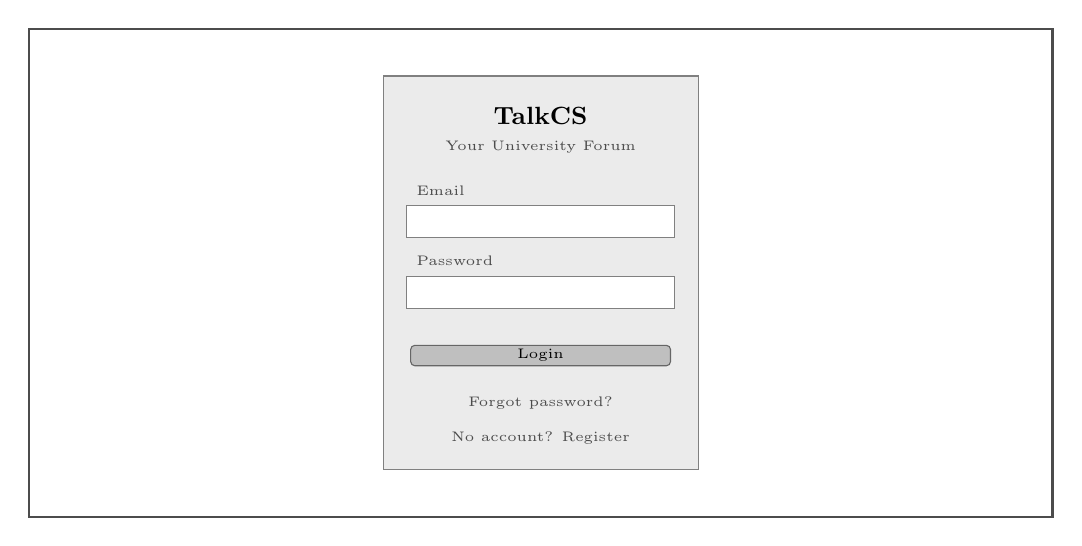
\begin{tikzpicture}[scale=1]
    \draw[frame] (0,0) rectangle (13,6.2);
    \draw[blk] (4.5,0.6) rectangle (8.5,5.6);
    \node[font=\small\bfseries] at (6.5,5.1) {TalkCS};
    \node[wtxt] at (6.5,4.7) {Your University Forum};
    \node[wtxt, anchor=west] at (4.8,4.15) {Email};
    \draw[fill=white, draw=black!50] (4.8,3.55) rectangle (8.2,3.95);
    \node[wtxt, anchor=west] at (4.8,3.25) {Password};
    \draw[fill=white, draw=black!50] (4.8,2.65) rectangle (8.2,3.05);
    \node[btn, minimum width=3.3cm] at (6.5,2.05) {Login};
    \node[wtxt] at (6.5,1.45) {Forgot password?};
    \node[wtxt] at (6.5,1.0) {No account? Register};
  \end{tikzpicture}
  \caption{Wireframe of the Login page}
  \label{fig:wf-login}
\end{figure}

\begin{figure}[H]
  \centering
  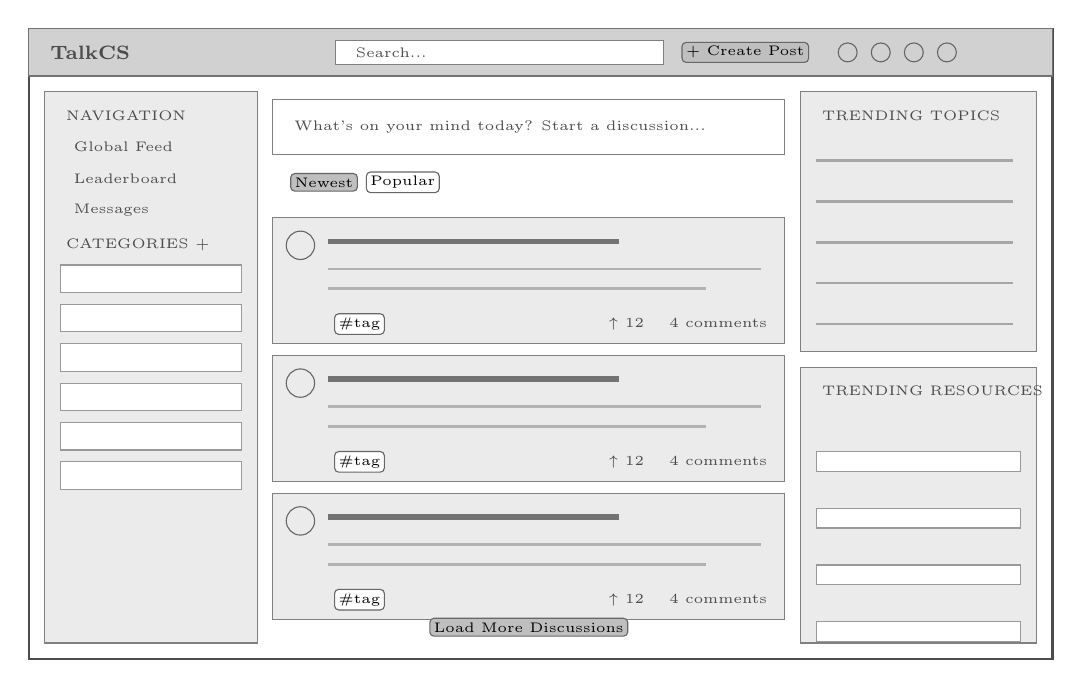
\begin{tikzpicture}
    \draw[frame] (0,0) rectangle (13,8);
    \wfnavbar{13}{8}
    % left sidebar
    \draw[blk] (0.2,0.2) rectangle (2.9,7.2);
    \node[wtxt, anchor=west] at (0.35,6.9) {NAVIGATION};
    \foreach \t [count=\i] in {Global Feed, Leaderboard, Messages} {\node[wtxt, anchor=west] at (0.45,6.9-\i*0.4) {\t};}
    \node[wtxt, anchor=west] at (0.35,5.25) {CATEGORIES \hfill +};
    \foreach \i in {1,...,6} {\draw[black!40, fill=white] (0.4,5.15-\i*0.5) rectangle (2.7,5.5-\i*0.5);}
    % center feed
    \draw[blk, fill=white] (3.1,6.4) rectangle (9.6,7.1);
    \node[wtxt, anchor=west] at (3.25,6.75) {What's on your mind today? Start a discussion...};
    \node[btn] at (3.75,6.05) {Newest}; \node[btn, fill=white] at (4.75,6.05) {Popular};
    \foreach \i in {0,1,2} {
      \draw[blk] (3.1,4.0-\i*1.75) rectangle (9.6,5.6-\i*1.75);
      \draw[black!60] (3.45,5.25-\i*1.75) circle (0.18);
      \draw[black!55, line width=2pt] (3.8,5.3-\i*1.75) -- (7.5,5.3-\i*1.75);
      \draw[black!30, line width=1pt] (3.8,4.95-\i*1.75) -- (9.3,4.95-\i*1.75);
      \draw[black!30, line width=1pt] (3.8,4.7-\i*1.75) -- (8.6,4.7-\i*1.75);
      \node[btn, fill=white] at (4.2,4.25-\i*1.75) {\#tag};
      \node[wtxt, anchor=east] at (9.5,4.25-\i*1.75) {$\uparrow$ 12 \quad 4 comments};
    }
    \node[btn] at (6.35,0.4) {Load More Discussions};
    % right sidebar
    \draw[blk] (9.8,3.9) rectangle (12.8,7.2);
    \node[wtxt, anchor=west] at (9.95,6.9) {TRENDING TOPICS};
    \foreach \i in {1,...,5} {\draw[black!35, line width=1pt] (10.0,6.85-\i*0.52) -- (12.5,6.85-\i*0.52);}
    \draw[blk] (9.8,0.2) rectangle (12.8,3.7);
    \node[wtxt, anchor=west] at (9.95,3.4) {TRENDING RESOURCES};
    \foreach \i in {1,...,4} {\draw[black!40, fill=white] (10.0,3.35-\i*0.72) rectangle (12.6,2.85-\i*0.72+0.25);}
  \end{tikzpicture}
  \caption{Wireframe of the Home page}
  \label{fig:wf-home}
\end{figure}

\begin{figure}[H]
  \centering
  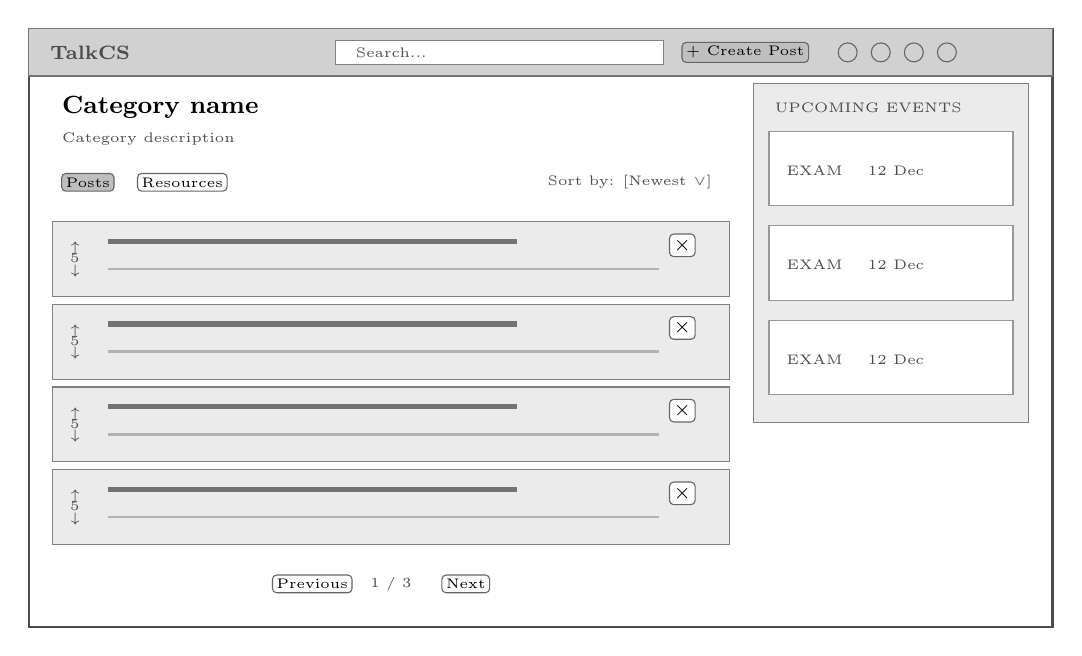
\begin{tikzpicture}
    \draw[frame] (0,0) rectangle (13,7.6);
    \wfnavbar{13}{7.6}
    \node[font=\small\bfseries, anchor=west] at (0.3,6.6) {Category name};
    \node[wtxt, anchor=west] at (0.3,6.2) {Category description};
    \node[btn] at (0.75,5.65) {Posts}; \node[btn, fill=white] at (1.95,5.65) {Resources};
    \node[wtxt, anchor=east] at (8.8,5.65) {Sort by: [Newest $\vee$]};
    \foreach \i in {0,1,2,3} {
      \draw[blk] (0.3,4.2-\i*1.05) rectangle (8.9,5.15-\i*1.05);
      \node[wtxt, anchor=west, align=left] at (0.4,4.67-\i*1.05) {$\uparrow$\\[-2pt]5\\[-2pt]$\downarrow$};
      \draw[black!55, line width=2pt] (1.0,4.9-\i*1.05) -- (6.2,4.9-\i*1.05);
      \draw[black!30, line width=1pt] (1.0,4.55-\i*1.05) -- (8.0,4.55-\i*1.05);
      \node[btn, fill=white] at (8.3,4.85-\i*1.05) {\scriptsize$\times$};
    }
    \node[btn, fill=white] at (3.6,0.55) {Previous}; \node[wtxt] at (4.6,0.55) {1 / 3}; \node[btn, fill=white] at (5.55,0.55) {Next};
    \draw[blk] (9.2,2.6) rectangle (12.7,6.9);
    \node[wtxt, anchor=west] at (9.35,6.6) {UPCOMING EVENTS};
    \foreach \i in {1,2,3} {\draw[black!40, fill=white] (9.4,6.55-\i*1.2) rectangle (12.5,6.55-\i*1.2+0.95);
      \node[wtxt, anchor=west] at (9.5,6.55-\i*1.2+0.45) {EXAM \quad 12 Dec};}
  \end{tikzpicture}
  \caption{Wireframe of the Category page}
  \label{fig:wf-category}
\end{figure}

\begin{figure}[H]
  \centering
  \begin{tikzpicture}
    \draw[frame] (0,0) rectangle (13,9);
    \wfnavbar{13}{9}
    \draw[blk] (0.3,5.2) rectangle (12.7,8.2);
    \node[wtxt, anchor=west, align=left] at (0.45,7.0) {$\uparrow$\\[-1pt]\small 12\\[-1pt]$\downarrow$};
    \draw[black!60, line width=3pt] (1.2,7.8) -- (8.0,7.8);
    \node[btn, fill=tcgreen] at (8.8,7.8) {SOLVED};
    \node[wtxt, anchor=west] at (1.2,7.45) {author \textbullet{} Lv.3 Regular \textbullet{} 2 days ago};
    \foreach \y in {7.0,6.7,6.4} {\draw[black!30, line width=1pt] (1.2,\y) -- (12.2,\y);}
    \draw[black!50, fill=black!12] (1.2,5.5) rectangle (8.0,6.2); \node[wtxt] at (4.6,5.85) {code block};
    \node[btn, fill=white] at (9.0,5.55) {\#java}; \node[btn, fill=white] at (10.0,5.55) {\#spring};
    \node[wtxt] at (12.3,7.8) {$\square$};
    \node[font=\scriptsize\bfseries, anchor=west] at (0.3,4.8) {Comments};
    \draw[fill=white, draw=black!50] (0.3,4.0) rectangle (12.7,4.5); \node[wtxt, anchor=west] at (0.4,4.25) {Write a comment...};
    \draw[blk, fill=tcgreen!50] (0.3,2.6) rectangle (12.7,3.75);
    \node[wtxt, anchor=west] at (0.4,3.5) {\checkmark{} Accepted Answer \quad answerer \textbullet{} Lv.2};
    \draw[black!30, line width=1pt] (0.9,3.1) -- (11.5,3.1);
    \node[wtxt, anchor=west] at (0.4,2.8) {$\uparrow$ 4 $\downarrow$ \quad Reply};
    \draw[blk] (1.3,1.5) rectangle (12.7,2.4);
    \draw[black!30, line width=1pt] (1.6,2.05) -- (11.0,2.05);
    \node[wtxt, anchor=west] at (1.4,1.7) {$\uparrow$ 1 $\downarrow$ \quad Reply \quad (nested reply)};
    \draw[blk] (0.3,0.3) rectangle (12.7,1.3);
    \draw[black!30, line width=1pt] (0.9,0.9) -- (11.0,0.9);
  \end{tikzpicture}
  \caption{Wireframe of the Post page}
  \label{fig:wf-post}
\end{figure}

\begin{figure}[H]
  \centering
  \begin{tikzpicture}
    \draw[frame] (0,0) rectangle (13,7.2);
    \wfnavbar{13}{7.2}
    \draw[blk] (0.2,0.2) rectangle (4.2,6.4);
    \node[font=\scriptsize\bfseries, anchor=west] at (0.35,6.1) {Messages};
    \draw[fill=white, draw=black!50] (0.35,5.4) rectangle (4.05,5.8); \node[wtxt, anchor=west] at (0.45,5.6) {Find user...};
    \foreach \i in {1,...,5} {
      \draw[black!40, fill=white] (0.35,5.3-\i*0.95) rectangle (4.05,5.3-\i*0.95+0.85);
      \draw[black!60] (0.7,5.3-\i*0.95+0.42) circle (0.2);
      \draw[black!55, line width=1.5pt] (1.05,5.3-\i*0.95+0.55) -- (2.6,5.3-\i*0.95+0.55);
      \draw[black!30, line width=1pt] (1.05,5.3-\i*0.95+0.27) -- (3.3,5.3-\i*0.95+0.27);
    }
    \node[circle, fill=tcorange, inner sep=1.2pt, font=\tiny, text=white] at (3.8,4.77) {2};
    \draw[blk] (4.4,0.2) rectangle (12.8,6.4);
    \draw[blkd] (4.4,5.8) rectangle (12.8,6.4); \node[wtxt, anchor=west] at (4.55,6.1) {other user};
    \foreach \y/\x/\w in {5.2/4.6/3.5, 4.5/8.9/3.7, 3.8/4.6/2.6, 3.1/9.6/3.0} {\draw[black!45, fill=white, rounded corners=3pt] (\x,\y-0.45) rectangle (\x+\w,\y);}
    \draw[fill=white, draw=black!50] (4.6,0.4) rectangle (11.9,0.95); \node[wtxt, anchor=west] at (4.7,0.67) {Type your message...};
    \node[btn] at (12.35,0.67) {$\triangleright$};
  \end{tikzpicture}
  \caption{Wireframe of the Chat page}
  \label{fig:wf-chat}
\end{figure}


% =====================================================================
\section{Directory Structure}

The repository is a monorepo containing both parts of the application.
Table~\ref{tab:dirs} describes the top-level structure, and Code~\ref{lst:tree} shows
the source layout in more detail.

\begin{table}[H]
  \centering
  \small
  \begin{tabularx}{\textwidth}{@{}l X@{}}
    \toprule
    \textbf{Path} & \textbf{Content} \\
    \midrule
    \code{backend/} & Spring Boot application (Gradle project) \\
    \code{backend/src/main/java/} & Java source code, package \code{com.talkcs.backend} \\
    \code{backend/src/main/resources/} & \code{application.properties} configuration \\
    \code{backend/src/test/} & JUnit tests and the test configuration \\
    \code{backend/uploads/} & Uploaded resources and avatars (created at runtime, not versioned) \\
    \code{backend/nixpacks.toml} & Build and start commands for deployment \\
    \code{frontend/} & React application (npm project) \\
    \code{frontend/src/} & TypeScript source code and tests \\
    \code{frontend/vercel.json} & SPA routing configuration for deployment \\
    \code{start.sh} & Starts backend and frontend together \\
    \code{test.sh} & Runs all backend and frontend tests \\
    \code{.env} & Local secrets (not versioned) \\
    \bottomrule
  \end{tabularx}
  \caption{Top-level directory structure}
  \label{tab:dirs}
\end{table}

\begin{lstlisting}[language={},numbers=none,caption={Source code layout},label={lst:tree}]
backend/src/main/java/com/talkcs/backend/
  BackendApplication.java   entry point, enables scheduling
  config/                   SecurityConfig, WebSocketConfig,
                            GlobalExceptionHandler, BadgeInitializer
  controller/               14 REST controllers
  dto/                      request and response objects
  model/                    20 JPA entities and enums
  repository/               Spring Data JPA repositories
  security/                 JwtUtils, JwtAuthFilter, UserLoader,
                            WebSocketAuthInterceptor
  service/                  20 services with the business logic

frontend/src/
  api/                      Axios client and one module per resource
  components/               Navbar, composer, editor, notification bell, ...
  components/ui/            reusable primitives (button, dialog, calendar, ...)
  context/                  Auth, Theme and UI context providers
  hooks/                    WebSocket subscription hooks
  lib/                      utility functions
  pages/                    one component per route
  App.tsx, main.tsx         routing and application bootstrap
\end{lstlisting}

% =====================================================================
\section{Design}

\subsection{Database and Persistence}

All persistent data is stored in PostgreSQL. The schema is not maintained by hand:
it is derived from the JPA entity classes, and Hibernate creates missing tables and
columns at start-up (\code{ddl-auto=update}). Primary keys are generated by the
database (\code{GenerationType.IDENTITY}), and all relations are mapped as lazily loaded
\code{@ManyToOne} associations, so related objects are fetched only when they are
actually needed.

Integrity rules are enforced on two levels. Unique constraints in the database
guarantee, for example, that a user can vote on a given post only once, can follow
another user only once, and can earn a badge only once. Business rules that cannot be
expressed as constraints, such as \emph{``users cannot vote on their own content''} or
\emph{``only the question author may accept an answer''}, are checked in the service
layer.

\subsection{Entity-Relationship Diagram}

Figure~\ref{fig:er} shows the entities of the database and their relations. For
readability, only the primary keys, foreign keys and the most important attributes are
shown; the complete column lists are given in Section~\ref{sec:tables}.

\begin{figure}[p]
  \centering
  % Entity-relationship diagram, drawn in two parts for readability.
\tikzset{
  entity/.style={rectangle split, rectangle split parts=2, draw=black!70, thick,
    rectangle split part fill={tcorange!85, white}, text width=3.1cm,
    font=\scriptsize\linespread{1.0}\selectfont, anchor=north, inner sep=3pt,
    rectangle split part align={center, left}},
  fk/.style={-{Stealth[length=2mm]}, thick, black!70, rounded corners=3pt},
  ufk/.style={-{Stealth[length=2mm]}, thick, tcbluedark!70, rounded corners=3pt},
}
\newcommand{\ent}[3]{\textbf{\textcolor{white}{#1}}\nodepart{two}#2}
\newcommand{\pk}[1]{\underline{#1}\ \textcolor{tcorange}{\tiny PK}}
\newcommand{\fkk}[1]{#1\ \textcolor{tcbluedark}{\tiny FK}}

\begin{subfigure}{\textwidth}
\centering
\resizebox{0.95\textwidth}{!}{%
\begin{tikzpicture}
  % Row 1
  \node[entity] (bm) at (1.7,0) {\ent{bookmarks}{\pk{id}\\\fkk{user\_id}\\\fkk{post\_id}\\created\_at}{}};
  \node[entity] (us) at (7.55,0) {\ent{users}{\pk{id}\\username \textcolor{tcgray}{\tiny U}\\email \textcolor{tcgray}{\tiny U}\\password (BCrypt)\\role\\reputation\\bio, avatar\_url\\created\_at}{}};
  \node[entity] (cr) at (13.4,0) {\ent{category\_reputations}{\pk{id}\\\fkk{user\_id}\\\fkk{category\_id}\\reputation}{}};
  % Row 2
  \node[entity] (po) at (1.7,-4.3) {\ent{posts}{\pk{id}\\title, body\\status\\\fkk{user\_id}\\\fkk{category\_id}\\\fkk{accepted\_answer\_id}\\created\_at}{}};
  \node[entity] (co) at (5.6,-4.3) {\ent{comments}{\pk{id}\\body\\\fkk{user\_id}\\\fkk{post\_id}\\\fkk{parent\_id}\\created\_at}{}};
  \node[entity] (vo) at (9.5,-4.3) {\ent{votes}{\pk{id}\\value ($\pm 1$)\\\fkk{user\_id}\\\fkk{post\_id}\\\fkk{comment\_id}\\\fkk{resource\_id}}{}};
  \node[entity] (re) at (13.4,-4.3) {\ent{resources}{\pk{id}\\title, description\\file\_name, file\_type\\file\_size, file\_path\\\fkk{user\_id}\\\fkk{category\_id}\\created\_at}{}};
  % Row 3
  \node[entity] (pt) at (1.7,-9.2) {\ent{post\_tags}{\fkk{\pk{post\_id}}\\\fkk{\pk{tag\_id}}}{}};
  \node[entity] (ta) at (5.6,-9.2) {\ent{tags}{\pk{id}\\name \textcolor{tcgray}{\tiny U}}{}};
  \node[entity] (ca) at (13.4,-9.2) {\ent{categories}{\pk{id}\\name \textcolor{tcgray}{\tiny U}\\description\\archived}{}};

  % references to users (blue)
  \draw[ufk] (bm.east |- 0,-0.9) -- (us.west |- 0,-0.9);
  \draw[ufk] (cr.west |- 0,-0.9) -- (us.east |- 0,-0.9);
  \draw[ufk] (po.north) -- (po.north |- 0,-3.6) -| ([xshift=-1.2cm]us.south);
  \draw[ufk] (co.north) -- ([xshift=-0.4cm]us.south);
  \draw[ufk] (vo.north) -- ([xshift=0.4cm]us.south);
  \draw[ufk] (re.north) -- (re.north |- 0,-3.6) -| ([xshift=1.2cm]us.south);
  % other references
  \draw[fk] (bm.south) -- (po.north -| bm.south) ;
  \draw[fk] (co.west |- 0,-5.4) -- (po.east |- 0,-5.4);
  \draw[fk] (po.east |- 0,-6.2) -- (co.west |- 0,-6.2);
  \draw[fk] (vo.west |- 0,-5.6) -- (co.east |- 0,-5.6);
  \draw[fk] (vo.east |- 0,-5.6) -- (re.west |- 0,-5.6);
  \draw[fk] (vo.south) -- ++(0,-0.55) -| ([xshift=0.6cm]po.south);
  \draw[fk] ([xshift=-0.6cm]pt.north) -- ([xshift=-0.6cm]po.south);
  \draw[fk] (pt.east |- 0,-9.75) -- (ta.west |- 0,-9.75);
  \draw[fk] (re.south) -- (ca.north);
  \draw[fk] (po.south) -- ++(0,-0.85) -| ([xshift=-0.8cm]ca.north);
  \draw[fk] (cr.east) -- ++(0.45,0) |- (ca.east);
  % self reference of comments
  \draw[fk] ([xshift=1.0cm]co.south) -- ++(0,-0.35) -- ++(0.65,0) |- ([yshift=-0.9cm]co.east);
  \node[font=\tiny, anchor=west] at ([xshift=1.0cm, yshift=-0.25cm]co.south) {parent};
\end{tikzpicture}}
\caption{Forum content: users, categories, posts, comments, tags, votes and resources}
\label{fig:er-a}
\end{subfigure}

\vspace{0.3cm}

\begin{subfigure}{\textwidth}
\centering
\resizebox{0.86\textwidth}{!}{%
\begin{tikzpicture}
  % Row 1
  \node[entity] (fo) at (1.7,0) {\ent{follows}{\pk{id}\\\fkk{follower\_id}\\\fkk{following\_id}\\created\_at}{}};
  \node[entity] (no) at (5.6,0) {\ent{notifications}{\pk{id}\\\fkk{recipient\_id}\\type, message\\link, is\_read\\created\_at}{}};
  \node[entity] (pr) at (9.5,0) {\ent{password\_reset\_tokens}{\pk{id}\\token \textcolor{tcgray}{\tiny U}\\\fkk{user\_id}\\expires\_at, used}{}};
  \node[entity] (sc) at (13.4,0) {\ent{site\_config}{\pk{id} (=1)\\site\_name, site\_tagline\\primary\_color, logo\_url}{}};
  % Row 2
  \node[entity] (cc) at (1.7,-3.6) {\ent{chat\_conversations}{\pk{id}\\\fkk{user\_a\_id}\\\fkk{user\_b\_id}\\last\_message\_at}{}};
  \node[entity] (us) at (7.55,-3.6) {\ent{users}{\pk{id}\\username, email, \dots}{}};
  \node[entity] (ub) at (13.4,-3.6) {\ent{user\_badges}{\pk{id}\\\fkk{user\_id}\\\fkk{badge\_id}\\awarded\_at}{}};
  % Row 3
  \node[entity] (cm) at (1.7,-7.0) {\ent{chat\_messages}{\pk{id}\\\fkk{conversation\_id}\\\fkk{sender\_id}\\\fkk{recipient\_id}\\content, sent\_at\\is\_read}{}};
  \node[entity] (ce) at (5.6,-7.0) {\ent{calendar\_events}{\pk{id}\\title, description\\start\_date, end\_date\\event\_type, is\_public\\\fkk{category\_id}\\\fkk{created\_by\_id}}{}};
  \node[entity] (cp) at (9.5,-7.0) {\ent{calendar\_event\_proposals}{\pk{id}\\title, description, dates\\event\_type, status\\admin\_note\\\fkk{category\_id}\\\fkk{submitted\_by\_id}}{}};
  \node[entity] (ba) at (13.4,-7.0) {\ent{badges}{\pk{id}\\name \textcolor{tcgray}{\tiny U}\\description, icon\_key\\type}{}};
  % Row 4
  \node[entity] (ca) at (7.55,-11.0) {\ent{categories}{\pk{id}\\name, \dots}{}};

  \draw[ufk] (fo.south) -- (fo.south |- 0,-2.9) -| ([xshift=-1.0cm]us.north);
  \draw[ufk] (no.south) -- (no.south |- 0,-3.2) -| ([xshift=-0.3cm]us.north);
  \draw[ufk] (pr.south) -- (pr.south |- 0,-3.2) -| ([xshift=0.3cm]us.north);
  \draw[ufk] (cc.east |- 0,-4.3) -- (us.west |- 0,-4.3);
  \draw[ufk] (ub.west |- 0,-4.3) -- (us.east |- 0,-4.3);
  \draw[ufk] (cm.east |- 0,-8.2) -- ++(0.25,0) |- ([yshift=-0.2cm]us.west |- 0,-4.65) -- (us.west |- 0,-4.65);
  \draw[ufk] (ce.north) -- ([xshift=-0.5cm]us.south);
  \draw[ufk] (cp.north) -- ([xshift=0.5cm]us.south);
  \draw[fk] (cm.north) -- (cc.south);
  \draw[fk] (ub.south) -- (ba.north);
  \draw[fk] (ce.south) -- (ce.south |- 0,-10.4) -| ([xshift=-0.5cm]ca.north);
  \draw[fk] (cp.south) -- (cp.south |- 0,-10.4) -| ([xshift=0.5cm]ca.north);
\end{tikzpicture}}
\caption{Community and system: following, notifications, chat, badges, calendar, configuration}
\label{fig:er-b}
\end{subfigure}

  \caption{Entity-relationship diagram of the TalkCS database}
  \label{fig:er}
\end{figure}

\subsection{Tables and Schema}
\label{sec:tables}

This section describes every table of the database. Column names follow Hibernate's
default naming strategy, which converts the camel-case field names of the entities to
snake case. \textbf{PK} marks primary keys, \textbf{FK} foreign keys, and \textbf{U}
unique columns or column groups.

\newcommand{\dbtable}[3]{%
  \begin{table}[H]
    \centering\small
    \begin{tabularx}{\textwidth}{@{}p{0.29\textwidth} p{0.17\textwidth} X@{}}
      \toprule
      \textbf{Column} & \textbf{Type} & \textbf{Description} \\
      \midrule
      #3
      \bottomrule
    \end{tabularx}
    \caption{The \texttt{#2} table}
    \label{tab:db-#1}
  \end{table}}

\subsubsection*{Users and Authentication}

\dbtable{users}{users}{
  id (PK) & bigint & Identifier of the user \\
  username & varchar & Unique display name, used for mentions and profile URLs \\
  email & varchar & Unique e-mail address, used for login and as JWT subject \\
  password & varchar & BCrypt hash of the password \\
  role & varchar & \code{STUDENT}, \code{PROFESSOR} or \code{ADMIN} \\
  reputation & integer & Total reputation (default 0) \\
  email\_notifications\_enabled & boolean & Whether e-mails are sent (default true) \\
  bio & text & Short self-description \\
  avatar\_url & varchar & Stored file name of the avatar image \\
  created\_at & timestamp & Time of registration \\
}

\dbtable{password_reset_tokens}{password\_reset\_tokens}{
  id (PK) & bigint & Identifier \\
  token (U) & varchar & Random UUID sent in the reset link \\
  user\_id (FK) & bigint & User who requested the reset \\
  expires\_at & timestamp & Expiry time (one hour after creation) \\
  used & boolean & Whether the token has already been used \\
}

\subsubsection*{Forum Content}

\dbtable{categories}{categories}{
  id (PK) & bigint & Identifier \\
  name (U) & varchar & Name of the subject or course \\
  description & varchar & Short description \\
  archived & boolean & Soft-deletion flag (default false) \\
  created\_at & timestamp & Creation time \\
}

\dbtable{posts}{posts}{
  id (PK) & bigint & Identifier \\
  title & varchar & Title of the question or discussion \\
  body & text & Markdown content \\
  user\_id (FK) & bigint & Author \\
  category\_id (FK) & bigint & Category of the post \\
  status & varchar & \code{OPEN}, \code{SOLVED} or \code{CLOSED} (default \code{OPEN}) \\
  accepted\_answer\_id (FK) & bigint & Accepted comment, if any \\
  created\_at & timestamp & Creation time \\
}

\dbtable{comments}{comments}{
  id (PK) & bigint & Identifier \\
  body & text & Markdown content \\
  user\_id (FK) & bigint & Author \\
  post\_id (FK) & bigint & Post the comment belongs to \\
  parent\_id (FK) & bigint & Parent comment for replies; \code{NULL} for root comments \\
  created\_at & timestamp & Creation time \\
}

\dbtable{tags}{tags}{
  id (PK) & bigint & Identifier \\
  name (U) & varchar & Normalized (lower-case) tag name \\
}

\dbtable{post_tags}{post\_tags}{
  post\_id (PK, FK) & bigint & Tagged post \\
  tag\_id (PK, FK) & bigint & Tag \\
}

\dbtable{resources}{resources}{
  id (PK) & bigint & Identifier \\
  title & varchar & Title given by the uploader \\
  description & varchar & Optional description \\
  file\_name & varchar & Original file name \\
  file\_type & varchar & MIME type \\
  file\_size & bigint & Size in bytes \\
  file\_path & varchar & Storage path on the server \\
  user\_id (FK) & bigint & Uploader \\
  category\_id (FK) & bigint & Category of the resource \\
  created\_at & timestamp & Upload time \\
}

\subsubsection*{Voting, Reputation and Badges}

\dbtable{votes}{votes}{
  id (PK) & bigint & Identifier \\
  value & integer & $+1$ (up-vote) or $-1$ (down-vote) \\
  user\_id (FK) & bigint & Voter \\
  post\_id (FK) & bigint & Voted post, or \code{NULL} \\
  comment\_id (FK) & bigint & Voted comment, or \code{NULL} \\
  resource\_id (FK) & bigint & Voted resource, or \code{NULL} (cascade on delete) \\
  created\_at & timestamp & Time of the vote \\
  \multicolumn{3}{@{}l}{\textit{U: (user\_id, post\_id), (user\_id, comment\_id), (user\_id, resource\_id)}} \\
}

\dbtable{category_reputations}{category\_reputations}{
  id (PK) & bigint & Identifier \\
  user\_id (FK) & bigint & User \\
  category\_id (FK) & bigint & Category \\
  reputation & integer & Reputation of the user within the category \\
  \multicolumn{3}{@{}l}{\textit{U: (user\_id, category\_id)}} \\
}

\dbtable{badges}{badges}{
  id (PK) & bigint & Identifier \\
  name (U) & varchar & Name of the badge, e.g. \emph{Rising Star} \\
  description & varchar & What the badge is awarded for \\
  icon\_key & varchar & Key selecting the icon in the frontend \\
  type & varchar & \code{MILESTONE} or \code{SPECIAL} \\
}

\dbtable{user_badges}{user\_badges}{
  id (PK) & bigint & Identifier \\
  user\_id (FK) & bigint & User who earned the badge \\
  badge\_id (FK) & bigint & Earned badge \\
  awarded\_at & timestamp & Time of the award \\
  \multicolumn{3}{@{}l}{\textit{U: (user\_id, badge\_id)}} \\
}

\subsubsection*{Social Features}

\dbtable{follows}{follows}{
  id (PK) & bigint & Identifier \\
  follower\_id (FK) & bigint & User who follows \\
  following\_id (FK) & bigint & User who is followed \\
  created\_at & timestamp & Time of following \\
  \multicolumn{3}{@{}l}{\textit{U: (follower\_id, following\_id)}} \\
}

\dbtable{bookmarks}{bookmarks}{
  id (PK) & bigint & Identifier \\
  user\_id (FK) & bigint & User \\
  post\_id (FK) & bigint & Bookmarked post \\
  created\_at & timestamp & Time of bookmarking \\
  \multicolumn{3}{@{}l}{\textit{U: (user\_id, post\_id)}} \\
}

\dbtable{notifications}{notifications}{
  id (PK) & bigint & Identifier \\
  recipient\_id (FK) & bigint & Notified user \\
  type & varchar & \code{MENTION}, \code{REPLY}, \code{VOTE\_MILESTONE}, \code{ACCEPTED\_ANSWER} or \code{FOLLOW} \\
  message & varchar & Text shown to the user \\
  link & varchar & Relative URL of the related page \\
  is\_read & boolean & Whether the notification has been read \\
  created\_at & timestamp & Creation time \\
}

\dbtable{chat_conversations}{chat\_conversations}{
  id (PK) & bigint & Identifier \\
  user\_a\_id (FK) & bigint & Participant with the smaller ID \\
  user\_b\_id (FK) & bigint & Participant with the larger ID \\
  last\_message\_at & timestamp & Time of the last message, used for ordering \\
  \multicolumn{3}{@{}l}{\textit{U: (user\_a\_id, user\_b\_id)}} \\
}

\dbtable{chat_messages}{chat\_messages}{
  id (PK) & bigint & Identifier \\
  conversation\_id (FK) & bigint & Conversation \\
  sender\_id (FK) & bigint & Sender \\
  recipient\_id (FK) & bigint & Recipient \\
  content & text & Message text \\
  sent\_at & timestamp & Time of sending \\
  is\_read & boolean & Whether the recipient has read the message \\
}

\subsubsection*{Calendar and Configuration}

\dbtable{calendar_events}{calendar\_events}{
  id (PK) & bigint & Identifier \\
  title & varchar & Title \\
  description & varchar & Optional description \\
  start\_date, end\_date & date & First and last day of the event \\
  event\_type & varchar & \code{EXAM}, \code{DEADLINE}, \code{LECTURE} or \code{OTHER} \\
  category\_id (FK) & bigint & Optional related category \\
  created\_by\_id (FK) & bigint & Creator \\
  is\_public & boolean & Visible to everyone (true) or only to the creator (false) \\
  created\_at & timestamp & Creation time \\
}

\dbtable{calendar_event_proposals}{calendar\_event\_proposals}{
  id (PK) & bigint & Identifier \\
  title, description & varchar & Proposed title and description \\
  start\_date, end\_date & date & Proposed dates \\
  event\_type & varchar & Proposed event type \\
  category\_id (FK) & bigint & Optional related category \\
  submitted\_by\_id (FK) & bigint & Proposing user \\
  status & varchar & \code{PENDING}, \code{APPROVED} or \code{REJECTED} \\
  admin\_note & varchar & Optional note of the reviewer \\
  created\_at & timestamp & Submission time \\
}

\dbtable{site_config}{site\_config}{
  id (PK) & bigint & Always 1 (single-row table) \\
  site\_name & varchar & Name of the installation (default \emph{TalkCS}) \\
  site\_tagline & varchar & Tagline (default \emph{University Forum Platform}) \\
  primary\_color & varchar & Primary colour (default \code{\#f97316}) \\
  logo\_url & varchar & URL of a custom logo \\
}


\subsection{Use Case Diagram}

Figure~\ref{fig:usecase} shows the main use cases of the three user roles. Because
the roles build on each other, a Professor can do everything a Student can, and an
Admin can do everything a Professor can; this is shown with generalization arrows.

\begin{figure}[htbp]
  \centering
  \resizebox{\textwidth}{!}{%
\begin{tikzpicture}[
    uc/.style={ellipse, draw=black!65, minimum width=4.4cm, minimum height=0.75cm, font=\scriptsize, inner sep=0.5pt, align=center},
    ucs/.style={uc, fill=tcblue!70},
    ucp/.style={uc, fill=tcgreen!90},
    uca/.style={uc, fill=tcorangelight},
    assoc/.style={black!50},
    gen/.style={-{Triangle[open, length=3mm, width=3mm]}, thick},
  ]
  \newcommand{\stick}[3]{%
    \begin{scope}[shift={(#1)}]
      \draw[thick, fill=white] (0,0.55) circle (0.22);
      \draw[thick] (0,0.33) -- (0,-0.35);
      \draw[thick] (-0.35,0.12) -- (0.35,0.12);
      \draw[thick] (0,-0.35) -- (-0.28,-0.85);
      \draw[thick] (0,-0.35) -- (0.28,-0.85);
      \node[font=\small\bfseries, fill=white, inner sep=1pt] at (0,-1.15) {#3};
      \coordinate (#2-l) at (-0.4,0.1);
      \coordinate (#2-r) at (0.4,0.1);
      \coordinate (#2-top) at (0,0.8);
      \coordinate (#2-bot) at (0,-1.4);
    \end{scope}}

  % ---------------- Student ----------------
  \foreach \i/\t in {0/Register and log in, 1/Reset password, 2/Create post with tags, 3/Comment and reply, 4/Vote on content, 5/Accept an answer, 6/Bookmark posts}
    \node[ucs] (sl\i) at (2.4, -\i*0.95) {\t};
  \foreach \i/\t in {0/Upload and download resources, 1/Search, 2/View profiles and leaderboard, 3/Follow users, 4/Chat with users, 5/Manage private events, 6/Propose public event}
    \node[ucs] (sr\i) at (11.6, -\i*0.95) {\t};
  \stick{7,-2.85}{S}{Student}
  \foreach \i in {0,...,6} { \draw[assoc] (S-l) -- (sl\i.east); \draw[assoc] (S-r) -- (sr\i.west); }

  % ---------------- Professor ----------------
  \foreach \i/\t in {0/Create and edit categories, 1/Publish public events}
    \node[ucp] (pl\i) at (2.4, -8.3-\i*0.95) {\t};
  \foreach \i/\t in {0/Review event proposals, 1/Delete any resource}
    \node[ucp] (pr\i) at (11.6, -8.3-\i*0.95) {\t};
  \stick{7,-8.85}{P}{Professor}
  \foreach \i in {0,1} { \draw[assoc] (P-l) -- (pl\i.east); \draw[assoc] (P-r) -- (pr\i.west); }

  % ---------------- Admin ----------------
  \foreach \i/\t in {0/View analytics, 1/Manage users and roles, 2/Configure branding}
    \node[uca] (al\i) at (2.4, -12.1-\i*0.95) {\t};
  \foreach \i/\t in {0/Archive and restore categories, 1/Delete any post or comment}
    \node[uca] (ar\i) at (11.6, -12.1-\i*0.95) {\t};
  \stick{7,-13.05}{A}{Admin}
  \foreach \i in {0,1,2} { \draw[assoc] (A-l) -- (al\i.east); }
  \foreach \i in {0,1} { \draw[assoc] (A-r) -- (ar\i.west); }

  % generalization: Professor -> Student, Admin -> Professor
  \draw[gen] (P-top) -- (S-bot);
  \draw[gen] (A-top) -- (P-bot);

\end{tikzpicture}}

  \caption{Use case diagram of TalkCS}
  \label{fig:usecase}
\end{figure}

\subsection{File Storage}

Uploaded files are stored on the local file system of the backend server. Resources are
saved in the \code{uploads/} directory, avatars in \code{uploads/avatars/}. To avoid
name collisions and path traversal through crafted file names, every file is stored
under a new name consisting of a random UUID followed by the original name. The
database stores the original file name, the MIME type, the size and the storage path.

Files are never served directly from the directory. Downloads go through
\code{GET /api/resources/\{id\}/download}, which looks up the resource, streams the
file, and sets the \code{Content-Type} and \code{Content-Disposition} headers so that
the browser saves the file under its original name. Avatars are likewise served
through \code{GET /api/users/\{username\}/avatar}. The maximum upload size is 50~MB,
configured through Spring's multipart settings.

% =====================================================================
\section{Backend Module Structure}

\subsection{Services}

Table~\ref{tab:services} summarizes the responsibility of each service.

\begin{longtable}{@{}p{0.30\textwidth} >{\raggedright\arraybackslash}p{0.65\textwidth}@{}}
  \toprule
  \textbf{Service} & \textbf{Responsibility} \\
  \midrule
  \endfirsthead
  \toprule
  \textbf{Service} & \textbf{Responsibility} \\
  \midrule
  \endhead
  \bottomrule
  \endfoot
  \bottomrule
  \caption{Backend services}
  \label{tab:services}
  \endlastfoot
  \code{AuthService} & Registration (uniqueness checks, BCrypt hashing) and login; issues JWTs \\
  \code{PasswordResetService} & Creates one-hour reset tokens, e-mails reset links, resets passwords \\
  \code{CategoryService} & CRUD of categories, soft deletion (archiving) and restoring \\
  \code{PostService} & Posts with pagination and sorting, tags, status, accepted answers, bookmarks, trending posts \\
  \code{CommentService} & Threaded comments built recursively; reply and mention notifications \\
  \code{VoteService} & Voting on posts, comments and resources; global and per-category reputation \\
  \code{ResourceService} & Upload, listing, download and deletion of resources; trending resources \\
  \code{SearchService} & Keyword search over posts, categories and users \\
  \code{SimilarityService} & BM25-based detection of similar posts \\
  \code{TagService} & Normalizing and creating tags; popular tags \\
  \code{TagSuggestionService} & Suggesting existing tags from post text \\
  \code{UserService} & Profiles, levels, avatars, leaderboard, follow system, user search \\
  \code{BadgeService} & Awarding milestone, accepted-answer and expertise badges \\
  \code{MentionService} & Extracting \code{@username} mentions from text \\
  \code{NotificationService} & Persisting notifications and triggering immediate e-mails \\
  \code{EmailService} & Building HTML e-mails and sending them through Resend \\
  \code{EmailDigestService} & Scheduled daily digest of unread notifications \\
  \code{ChatService} & Conversations, messages, unread counts, real-time delivery \\
  \code{CalendarService} & Events, visibility rules and the proposal workflow \\
  \code{AdminService} & Statistics, user management, anonymizing deletion, site configuration \\
\end{longtable}

\subsection{REST API}

All endpoints are located under the \url{/api} prefix, accept and return JSON (except
file uploads and downloads), and require a valid JWT unless marked as public.
Tables~\ref{tab:api1} and~\ref{tab:api2} list the endpoints.

{\small
\begin{longtable}{@{}>{\raggedright\arraybackslash}p{0.14\textwidth} p{0.44\textwidth} >{\raggedright\arraybackslash}p{0.36\textwidth}@{}}
  \toprule
  \textbf{Method} & \textbf{Path} & \textbf{Purpose} \\
  \midrule
  \endfirsthead
  \toprule
  \textbf{Method} & \textbf{Path} & \textbf{Purpose} \\
  \midrule
  \endhead
  \bottomrule
  \endfoot
  \bottomrule
  \caption{REST API: authentication, content and community}
  \label{tab:api1}
  \endlastfoot
  \multicolumn{3}{@{}l}{\textit{Authentication (public)}} \\
  POST & \url{/auth/register} & Register; returns a JWT \\
  POST & \url{/auth/login} & Log in; returns a JWT \\
  POST & \url{/auth/forgot-password} & Request a reset e-mail \\
  POST & \url{/auth/reset-password} & Set a new password with a token \\
  \multicolumn{3}{@{}l}{\textit{Categories}} \\
  GET & \url{/categories} & Active categories \\
  GET & \url{/categories/{id}} & One category \\
  GET & \url{/categories/admin/all} & All incl. archived (Admin) \\
  POST, PUT & \url{/categories}, \url{/categories/{id}} & Create / edit (Professor, Admin) \\
  DELETE & \url{/categories/{id}} & Archive (Admin) \\
  PUT & \url{/categories/{id}/restore} & Restore (Admin) \\
  \multicolumn{3}{@{}l}{\textit{Posts}} \\
  GET & \url{/posts?categoryId=\&page=\&size=\&sortBy=} & Paginated list; \code{sortBy} is \code{newest}, \code{votes} or \code{comments} \\
  POST & \url{/posts} & Create a post \\
  GET, PUT, DELETE & \url{/posts/{id}} & Read / edit (author) / delete (author, Admin) \\
  PUT & \url{/posts/{id}/status} & Set status (author, Admin) \\
  GET & \url{/posts/trending?limit=} & Trending posts of the last 7 days \\
  GET & \url{/posts/similar?title=\&body=\&categoryId=\&tags=} & Up to three similar posts \\
  PUT & \url{/posts/{id}/accept/{commentId}} & Accept an answer (author) \\
  DELETE & \url{/posts/{id}/accept} & Withdraw acceptance (author) \\
  POST, DELETE & \url{/posts/{id}/bookmark} & Bookmark / remove bookmark \\
  \multicolumn{3}{@{}l}{\textit{Comments, votes, tags}} \\
  GET & \url{/comments?postId=\&page=\&size=} & Root comments with nested replies \\
  POST & \url{/comments} & Create a comment or reply (\code{parentId}) \\
  PUT, DELETE & \url{/comments/{id}} & Edit (author) / delete (author, Admin) \\
  POST & \url{/votes/post/{id}}, \url{/votes/comment/{id}}, \url{/votes/resource/{id}} & Vote with value $+1$ or $-1$ \\
  GET & \url{/tags}, \url{/tags/popular} & All tags / 20 most used tags \\
  POST & \url{/tags/suggest} & Suggest tags for a title and body \\
  \multicolumn{3}{@{}l}{\textit{Resources and search}} \\
  GET & \url{/resources?categoryId=} & Resources of a category \\
  GET & \url{/resources/trending} & Most up-voted resources \\
  POST & \url{/resources} & Upload (multipart: file, title, description, categoryId) \\
  GET & \url{/resources/{id}/download} & Download the file (public) \\
  DELETE & \url{/resources/{id}} & Delete (uploader, Professor, Admin) \\
  GET & \url{/search?q=} & Search posts, categories, users (public) \\
\end{longtable}

\begin{longtable}{@{}>{\raggedright\arraybackslash}p{0.14\textwidth} p{0.44\textwidth} >{\raggedright\arraybackslash}p{0.36\textwidth}@{}}
  \toprule
  \textbf{Method} & \textbf{Path} & \textbf{Purpose} \\
  \midrule
  \endfirsthead
  \toprule
  \textbf{Method} & \textbf{Path} & \textbf{Purpose} \\
  \midrule
  \endhead
  \bottomrule
  \endfoot
  \bottomrule
  \caption{REST API: users, messaging, calendar and administration}
  \label{tab:api2}
  \endlastfoot
  \multicolumn{3}{@{}l}{\textit{Users}} \\
  GET & \url{/users/{username}} & Public profile (public) \\
  GET & \url{/users/{username}/posts} & Posts of a user (public) \\
  GET & \url{/users/{username}/avatar} & Avatar image (public) \\
  GET & \url{/users/leaderboard} & Top 20 users (public) \\
  GET & \url{/users/me} & Profile of the current user \\
  PUT & \url{/users/me}, \url{/users/me/avatar} & Update bio / upload avatar \\
  GET & \url{/users/search?q=} & Find users (for starting a chat) \\
  GET & \url{/users/{username}/bookmarks} & Bookmarked posts \\
  GET & \url{/users/{username}/badges} & Milestone and special badges \\
  POST, DELETE & \url{/users/{username}/follow} & Follow / unfollow \\
  \multicolumn{3}{@{}l}{\textit{Notifications and chat}} \\
  GET & \url{/notifications}, \url{/notifications/count} & List / unread count \\
  PUT & \url{/notifications/{id}/read}, \url{/notifications/read-all} & Mark as read \\
  GET & \url{/chat/conversations} & Conversations of the user \\
  POST & \url{/chat/conversations/open/{username}} & Open or create a conversation \\
  GET & \url{/chat/conversations/{id}/messages} & Messages; marks them read \\
  GET & \url{/chat/unread-count} & Number of unread messages \\
  \multicolumn{3}{@{}l}{\textit{Calendar}} \\
  GET & \url{/calendar?year=\&month=\&categoryId=} & Visible events of a month \\
  GET & \url{/calendar/upcoming?categoryId=\&limit=} & Next public events \\
  POST & \url{/calendar} & Create an event (public for Professor/Admin) \\
  PUT, DELETE & \url{/calendar/{id}} & Edit / delete (creator, Professor, Admin) \\
  POST & \url{/calendar/proposals} & Propose a public event \\
  GET & \url{/calendar/proposals/mine} & Own proposals \\
  GET & \url{/calendar/proposals} & Pending proposals (Professor, Admin) \\
  PUT & \url{/calendar/proposals/{id}/approve|reject} & Review a proposal (Professor, Admin) \\
  \multicolumn{3}{@{}l}{\textit{Administration (Admin only)}} \\
  GET & \url{/admin/stats} & Platform statistics \\
  GET & \url{/admin/users?page=\&search=} & Paginated user list \\
  PUT & \url{/admin/users/{id}/role} & Change role \\
  DELETE & \url{/admin/users/{id}} & Anonymize a user \\
  GET, PUT & \url{/admin/config} & Read / update branding \\
\end{longtable}
}

\subsection{Error Handling}

Errors are handled centrally by the \code{GlobalExceptionHandler}, annotated with
\code{@RestControllerAdvice}. Authorization failures
(\code{AccessDeniedException}) are translated to \code{403 Forbidden}, and business
rule violations, which the services signal with a \code{RuntimeException} and a
human-readable message, are translated to \code{400 Bad Request} with the message as
the response body. The frontend displays this message to the user. Requests without
valid authentication on a protected endpoint are answered by the security
configuration with \code{401 Unauthorized} and a JSON error body.

% =====================================================================
\section{Frontend Module Structure}

\subsection{Context Providers}

Global state is kept in three React contexts, mounted in \code{App.tsx} around the
router:

\begin{itemize}
  \item \code{AuthContext} holds the logged-in user and the token, restores them from
    \code{localStorage} on page load, and provides the \code{login} and \code{logout}
    functions and an \code{isAuthenticated} flag.
  \item \code{ThemeContext} stores the selected theme (dark, light or system) under the
    key \code{talkcs-ui-theme} and applies the corresponding class to the
    \code{<html>} element.
  \item \code{UIContext} controls the global post composer dialog, so that it can be
    opened from any page, optionally with a preselected category.
\end{itemize}

In addition, a TanStack Query \code{QueryClient} caches server data for five minutes
and retries failed requests once.

\subsection{Pages and Routing}

Each route of the application is implemented by one page component, as listed in
Table~\ref{tab:pages}. Routes that require authentication are wrapped in the
\code{ProtectedRoute} component, which redirects unauthenticated users to the login
page. Unknown paths redirect to the home page.

\begin{table}[H]
  \centering
  \small
  \begin{tabularx}{\textwidth}{@{}l l X c@{}}
    \toprule
    \textbf{Route} & \textbf{Component} & \textbf{Content} & \textbf{Auth} \\
    \midrule
    \route{/login}, \route{/register} & \code{LoginPage}, \code{RegisterPage} & Authentication forms & -- \\
    \route{/forgot-password} & \code{ForgotPasswordPage} & Request reset link & -- \\
    \route{/reset-password} & \code{ResetPasswordPage} & Set new password & -- \\
    \route{/} & \code{HomePage} & Global feed, categories, trending & \checkmark \\
    \route{/category/:id} & \code{CategoryPage} & Posts, resources, upcoming events & \checkmark \\
    \route{/post/:id} & \code{PostPage} & Post, threaded comments, voting & \checkmark \\
    \route{/profile/:username} & \code{ProfilePage} & Profile, posts, bookmarks & -- \\
    \route{/profile/:username/badges} & \code{BadgesPage} & Milestones, achievements & \checkmark \\
    \route{/search} & \code{SearchPage} & Search results & -- \\
    \route{/leaderboard} & \code{LeaderboardPage} & Top users & \checkmark \\
    \route{/chat} & \code{ChatPage} & Direct messaging & \checkmark \\
    \route{/calendar} & \code{CalendarPage} & Calendar and proposals & \checkmark \\
    \route{/admin} & \code{AdminPage} & Admin Panel & \checkmark \\
    \bottomrule
  \end{tabularx}
  \caption{Frontend routes and page components}
  \label{tab:pages}
\end{table}

\subsection{Shared Components}

\begin{itemize}
  \item \code{Navbar}: the top navigation bar with search, post creation, chat and
    notification indicators, theme toggle and the mobile menu.
  \item \code{GlobalPostComposer}: the post creation dialog with category selection,
    Markdown editor, tag input, tag suggestions and the debounced similar-post search.
  \item \code{MarkdownEditor}: a wrapper around \code{@uiw/react-md-editor} that follows
    the active theme.
  \item \code{NotificationBell}: the notification dropdown; it polls the unread count
    every 30 seconds.
  \item \code{ChatIcon}: the chat link with the unread message counter.
  \item \code{ProtectedRoute}, \code{ThemeToggle}, \code{NavbarSearch}.
  \item \code{components/ui}: accessible primitives (button, card, dialog, dropdown,
    select, popover, calendar, date-time picker) and the \code{EventManager} calendar
    component with month, week, day and list views.
\end{itemize}

\subsection{API Modules and Hooks}

The \code{api} directory contains one module per backend resource (\code{auth},
\code{posts}, \code{comments}, \code{votes}, \code{resources}, \code{users},
\code{chat}, \code{calendar}, \code{notifications}, \code{admin}, \code{badges},
\code{tags}, \code{categories}, \code{search}). Each module exports typed functions,
for example \code{getPosts(categoryId, page, size, sortBy)}, so components never build
URLs themselves. All modules share the Axios instance defined in \code{api.ts}
(Code~\ref{lst:axios}), whose base URL is read from the \code{VITE\_API\_URL}
environment variable.

\begin{lstlisting}[language=TypeScript,caption={Shared Axios instance with authentication interceptors (\texttt{api.ts}, abridged)},label={lst:axios}]
const api = axios.create({
  baseURL: import.meta.env.VITE_API_URL || 'http://localhost:8080',
});

// Attach the JWT to every request
api.interceptors.request.use((config) => {
  const token = localStorage.getItem('token');
  if (token) config.headers.Authorization = `Bearer ${token}`;
  return config;
});

// An expired or invalid token logs the user out
api.interceptors.response.use((r) => r, (error) => {
  if (error.response?.status === 401) {
    localStorage.removeItem('token');
    localStorage.removeItem('user');
    if (!window.location.pathname.includes('/login'))
      window.location.href = '/login';
  }
  return Promise.reject(error);
});
\end{lstlisting}

Two custom hooks encapsulate the WebSocket subscriptions for live updates:
\code{usePostUpdates(categoryId, onUpdate)} subscribes to
\code{/topic/category/\{id\}} and \code{useCommentUpdates(postId, onUpdate)} to
\code{/topic/post/\{id\}}. Both create a STOMP client when the component mounts and
deactivate it when it unmounts, so that no connection is left open after the user
leaves a page.

% =====================================================================
\section{Key Implementation Details}

\subsection{Token Generation and Validation}

JWTs are created and verified by the \code{JwtUtils} component
(Code~\ref{lst:jwt}). The token contains the user's e-mail address as subject and an
expiry time of 24 hours, and is signed with the HMAC-SHA key derived from the
Base64-encoded secret. Because the e-mail address is the subject, the
\code{UserLoader} (the application's \code{UserDetailsService}) looks users up by
e-mail and grants them the authority \code{ROLE\_<role>}.

\begin{lstlisting}[language=Java,caption={Creating and validating JWTs (\texttt{JwtUtils.java}, abridged)},label={lst:jwt}]
public String generateToken(String username) {
    return Jwts.builder()
        .subject(username)
        .issuedAt(new Date())
        .expiration(new Date(System.currentTimeMillis() + jwtExpirationMs))
        .signWith(getSigningKey())
        .compact();
}

public boolean validateToken(String token) {
    try {
        Jwts.parser().verifyWith(getSigningKey()).build()
            .parseSignedClaims(token);   // checks signature and expiry
        return true;
    } catch (Exception e) {
        return false;
    }
}

private SecretKey getSigningKey() {
    return Keys.hmacShaKeyFor(Decoders.BASE64.decode(jwtSecret));
}
\end{lstlisting}

Authorization is enforced at two levels. Role-based rules are declared on controller
methods, e.g. \code{@PreAuthorize("hasAnyRole('ADMIN', 'PROFESSOR')")}, or on a whole
controller, as in the case of \code{AdminController}. Ownership rules (``only the
author may edit this post'') depend on the data and are therefore checked in the
services by comparing the e-mail of the authenticated user with the owner of the
entity.

\subsection{Voting and Reputation}

A vote is stored as a \code{Vote} row with the value $+1$ or $-1$ and a reference to
exactly one target: a post, a comment or a resource. Unique constraints on
(\code{user\_id}, \code{post\_id}), (\code{user\_id}, \code{comment\_id}) and
(\code{user\_id}, \code{resource\_id}) make it impossible to vote twice on the same item.

The reputation of the author is updated incrementally instead of being recomputed from
all votes, which keeps voting a constant-time operation. Let $v \in \{+1,-1\}$ be the
new vote and $e$ the existing vote of the same user on the same target, if any. The
service distinguishes three cases:

\begin{itemize}
  \item no existing vote: a new vote is stored and the reputation changes by $v$;
  \item $e = v$ (the same arrow is clicked again): the vote is withdrawn, deleted, and
    the reputation changes by $-v$;
  \item $e \neq v$ (the opposite arrow is clicked): the vote is updated and the
    reputation changes by $v - e$, i.e. by $\pm 2$.
\end{itemize}

For posts and comments, the same change is applied to the \code{CategoryReputation} of
the author in the category of the post, which is created on demand
(Code~\ref{lst:vote}). After every vote, \code{BadgeService.checkExpertiseBadges}
checks whether the author has reached a new expertise threshold in that category.

\begin{lstlisting}[language=Java,caption={Applying a vote to a post (\texttt{VoteService.java}, abridged)},label={lst:vote}]
voteRepository.findByVoterIdAndPostId(voter.getId(), postId).ifPresentOrElse(
    existing -> {
        if (existing.getValue() == value) {          // toggle off
            author.setReputation(author.getReputation() - value);
            adjustCategoryRep(author, post.getCategory(), -value);
            voteRepository.delete(existing);
        } else {                                     // switch direction
            int delta = value - existing.getValue();
            author.setReputation(author.getReputation() + delta);
            adjustCategoryRep(author, post.getCategory(), delta);
            existing.setValue(value);
            voteRepository.save(existing);
        }
    },
    () -> {                                          // first vote
        author.setReputation(author.getReputation() + value);
        adjustCategoryRep(author, post.getCategory(), value);
        voteRepository.save(Vote.builder().voter(voter).post(post)
            .value(value).createdAt(LocalDateTime.now()).build());
    });
badgeService.checkExpertiseBadges(author, post.getCategory());
\end{lstlisting}

Accepting an answer adds 15 points to the answerer's global and category reputation
and 2 points to the question author; withdrawing the acceptance subtracts the global
points again, never letting the reputation fall below zero.

\subsection{Levels and Badges}

The level of a user is a pure function of the reputation $r$:

\begin{equation}
  \mathit{level}(r) =
  \begin{cases}
    1 \ (\text{Newcomer}) & \text{if } r < 50,\\
    2 \ (\text{Contributor}) & \text{if } 50 \le r < 200,\\
    3 \ (\text{Regular}) & \text{if } 200 \le r < 500,\\
    4 \ (\text{Trusted}) & \text{if } 500 \le r < 1000,\\
    5 \ (\text{Expert}) & \text{if } r \ge 1000.
  \end{cases}
\end{equation}

Levels are not stored but computed in \code{UserService} whenever a profile or a post
is returned, so they can never get out of sync with the reputation.

Badges are stored in the \code{badges} table and awarded through the \code{user\_badges}
join table. At start-up, the \code{BadgeInitializer} (a \code{CommandLineRunner})
inserts the twelve milestone badges if they do not exist yet. After a user creates a
post or a comment or receives an accepted answer, \code{BadgeService.checkAndAwardBadges}
compares the user's post count, comment count and reputation against the thresholds,
and awards every badge that has been reached but not yet earned. Expertise badges are
created dynamically, because their names contain the category name (for example
\emph{Databases Expert (Silver)}); the method \code{tryAward} looks the badge up by name,
creates it if necessary, and inserts the \code{UserBadge} row only if it does not exist.

\subsection{Similar Post Detection}
\label{sec:similarity}

Duplicate questions are one of the main problems of student group chats, so TalkCS
warns the author of a new post about existing similar posts while they are typing. The
frontend calls \code{GET /api/posts/similar} 500 milliseconds after the last keystroke
(debouncing), sending the current title, body, category and tags. The
\code{SimilarityService} compares the draft with every post of the selected category and
returns at most three posts whose score is at least 0.08.

\subsubsection*{Preprocessing}

Texts are converted to lower case and split into tokens at every character that is not
a letter, a digit, \code{\#} or \code{+} (so that terms such as \code{c++} and
\code{c\#} survive). Tokens of at most two characters and common English stop words
(\emph{the}, \emph{is}, \emph{how}, \dots) are discarded.

\subsubsection*{Scoring}

The final score of a candidate post $d$ for the draft $q$ is a weighted combination of
three signals:

\begin{equation}
  \mathit{score}(q,d) = 0.5 \cdot \frac{\mathrm{BM25}(q,d)}{\max_{d'} \mathrm{BM25}(q,d')}
    + 0.3 \cdot J(T_q, T_d) + 0.2 \cdot J(G_q, G_d)
  \label{eq:score}
\end{equation}

\noindent where $T_q, T_d$ are the sets of title tokens, $G_q, G_d$ are the sets of tags,
and $J(A,B) = |A \cap B| \,/\, |A \cup B|$ is the Jaccard similarity.

The first term is the Okapi BM25 ranking function~\cite{bm25}, a standard relevance measure
from information retrieval, which compares the tokens of the draft's title and body with
the body of each post:

\begin{equation}
  \mathrm{BM25}(q,d) = \sum_{t \in q} \mathrm{IDF}(t) \cdot
    \frac{f(t,d)\,(k_1 + 1)}{f(t,d) + k_1 \left(1 - b + b\,\frac{|d|}{\mathit{avgdl}}\right)}
\end{equation}

\begin{equation}
  \mathrm{IDF}(t) = \ln\!\left(\frac{N - n(t) + 0.5}{n(t) + 0.5} + 1\right)
\end{equation}

\noindent Here $f(t,d)$ is the number of occurrences of term $t$ in post $d$, $|d|$ is
the number of tokens of $d$, $\mathit{avgdl}$ is the average length of the posts in the
category, $N$ is the number of posts in the category and $n(t)$ is the number of posts
containing $t$. The parameters have the commonly used values $k_1 = 1.5$ and $b = 0.75$.

BM25 rewards posts that share rare, specific terms with the draft (for example
\emph{dijkstra} or \emph{segfault}) much more than posts sharing frequent terms, and the
length normalization prevents long posts from dominating. Because raw BM25 scores are
unbounded, they are normalized by the best score in the category, so all three terms of
Equation~\ref{eq:score} lie in $[0,1]$. Titles are compared separately because the title
of a question is usually its most concise summary, and tags capture the topic even when
two posts use different wording.

The approach needs no training data and no external service, works from the very first
post, and adapts automatically as the corpus of a category grows. Since the corpus is
restricted to one category, the computation stays fast for the expected size of a
university forum.

\subsection{Tag Suggestion}

\code{TagSuggestionService} applies the same tokenization to the title and body of a
draft and returns up to five existing tags such that a token of the text contains the
tag name, or the tag name contains a token. Suggesting only existing tags keeps the tag
vocabulary of the platform consistent. Tags themselves are normalized (trimmed and
converted to lower case) by \code{TagService} before they are looked up or created, so
\code{Java} and \code{java} refer to the same tag.

\subsection{Trending Posts and Resources}

The trending section of the home page is computed by a single JPQL query that ranks the
posts created in the last seven days by an activity score in which an up-vote counts
twice as much as a comment:

\begin{equation}
  \mathit{trending}(p) = 2 \cdot \mathit{upvotes}(p) + \mathit{comments}(p)
\end{equation}

Trending resources are ranked by the number of up-votes they received, with newer
resources first among equals.

\subsection{Threaded Comments and Live Updates}

Comments form a tree: every comment references its post and optionally a parent
comment. The comment endpoint pages only the root comments of a post
(\code{findByPostIdAndParentIsNull}); the replies of each comment are loaded recursively
by \code{CommentService.getChildren} and returned as a nested \code{children} list. The
frontend renders this structure with a recursive component.

When a comment is created, edited or deleted, the \code{CommentController} publishes a
small event to \code{/topic/post/\{postId\}} (Code~\ref{lst:broadcast}). Every browser
displaying that post receives the event through the \code{useCommentUpdates} hook and
refetches the comments. Posts in a category are kept up to date in the same way through
\code{/topic/category/\{categoryId\}}.

\begin{lstlisting}[language=Java,caption={Broadcasting a new comment (\texttt{CommentController.java})},label={lst:broadcast}]
@PostMapping
public ResponseEntity<CommentResponse> createComment(
        @Valid @RequestBody CommentRequest request) {
    CommentResponse response = commentservice.createComment(request);
    messagingTemplate.convertAndSend("/topic/post/" + request.getPostId(),
            (Object) Map.of("action", "created", "comment", response));
    return ResponseEntity.ok(response);
}
\end{lstlisting}

\subsection{Direct Messaging}

A conversation is stored once for every pair of users. To guarantee this, the
participant with the smaller ID is always stored as \code{userA} and the other as
\code{userB}, and the pair is protected by a unique constraint; opening a conversation
therefore either finds the existing row or creates a new one. A message stores its
sender, its recipient and a read flag, which makes counting unread messages per
conversation and per user a simple query.

Messages are sent over STOMP to \code{/app/chat.send}. The \code{ChatService} checks that
the sender is a participant of the conversation, persists the message, updates the time
of the last message, and publishes the message to the private topics of both
participants, so that the sender's other open tabs are updated as well.

\subsection{Notifications and E-mails}

The \code{NotificationService} is called by other services whenever something happens
that a user should know about: a reply to their post, a mention, an accepted answer, or
a new follower. Mentions are extracted by \code{MentionService} with the regular
expression \code{@(\textbackslash w+)}; each distinct username that belongs to an existing
user (other than the author) is notified. Every notification is stored in the database;
mentions and accepted answers additionally trigger an immediate HTML e-mail through
\code{EmailService}, unless the user has disabled e-mail notifications.

The daily digest is implemented with Spring's task scheduling
(Code~\ref{lst:digest}). Scheduling is enabled on the application class with
\code{@EnableScheduling}, and the job runs every weekday at 8:00 server time. Failures to
send an e-mail are logged but never interrupt the operation that triggered them.

\begin{lstlisting}[language=Java,caption={Scheduled daily digest (\texttt{EmailDigestService.java}, abridged)},label={lst:digest}]
@Scheduled(cron = "0 0 8 * * MON-FRI")
public void sendDailyDigests() {
    LocalDateTime since = LocalDateTime.now().minusHours(24);
    userRepository.findAll().stream()
        .filter(User::isEmailNotificationsEnabled)
        .forEach(user -> sendDigestForUser(user, since));
}
\end{lstlisting}

\subsection{Calendar Visibility and Proposals}

Each event has a \code{publicEvent} flag. When the events of a month are requested, the
service returns the public events of that month together with the private events
created by the requesting user, optionally filtered by category, sorted by start date.
Events created directly by professors and administrators are public; events created by
students are private. A student who wants to publish an event submits a
\code{CalendarEventProposal} with status \code{PENDING}. Approving it creates a new
public event from the proposal data and sets the status to \code{APPROVED} in one
transaction; rejecting it sets the status to \code{REJECTED} and stores the optional
reviewer note.

\subsection{Password Reset}

A password reset request deletes all previous tokens of the user and creates a new
random UUID token valid for one hour. The token is sent in a link to the
\route{/reset-password} page; the link is built from the configured frontend URL
(\code{app.base-url}). When the new password is submitted, it must be at least
8 characters long, as at registration, and the token must exist,
must not have been used, and must not have expired; the password is then hashed with
BCrypt and the token is marked as used, so it cannot be used again. If the e-mail address
is not registered, the request silently succeeds, which prevents attackers from
discovering registered addresses.

\subsection{Soft Deletion}

Two kinds of data are never physically deleted, in order to keep existing discussions
consistent. Categories are \emph{archived}: an \code{archived} flag hides them from the
public category list, and they can be restored at any time. Deleted users are
\emph{anonymized}: their username and e-mail are replaced by
\code{deleted\_user\_<id>} and \code{deleted\_<id>@deleted.invalid}, and their password,
bio and avatar are removed. Their posts and comments stay in place, attributed to the
anonymized account, but the account can no longer be used to log in.
